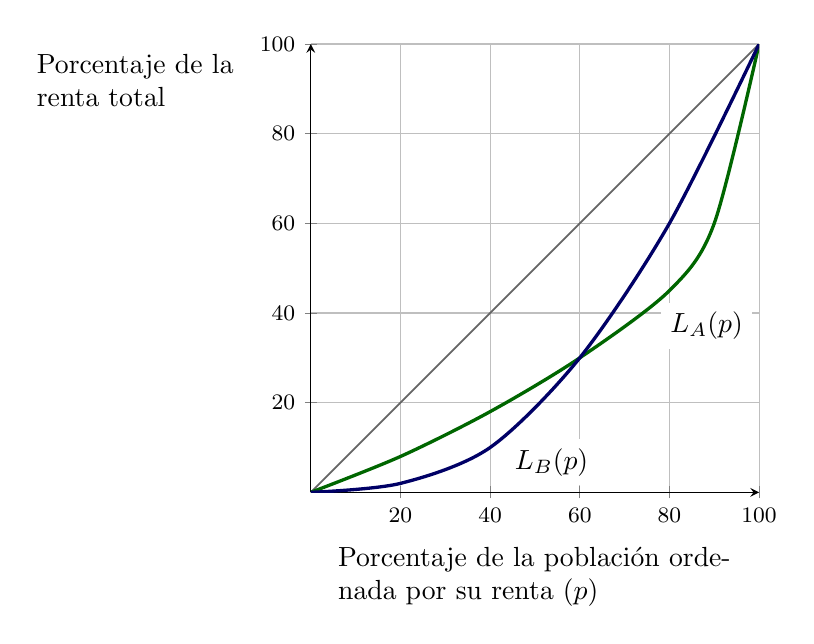
\begin{tikzpicture}
  \begin{axis}[
    axis equal image = true,
    axis lines = middle,
    x label style={at={(axis description cs:0.5, -0.1)},
      anchor=north, text width = 5cm},
    y label style={at={(axis description cs:-0.15, 1)},
      anchor=north east, text width = 2.5 cm},
    xlabel={Porcentaje de la población ordenada por su renta ($p$)},
    ylabel={Porcentaje de la renta total},
    xmin=0, xmax=100, ymin=0, ymax=100,
    ticklabel style = {font=\footnotesize},
    xtick={0, 20, 40, 60, 80, 100},
    ytick={0, 20, 40, 60, 80, 100},
    % legend pos=south east,
    grid=major
    ]
    % Línea de igualdad perfecta
    \addplot[domain=0:100, semithick, black!60!] {x} ;

    % Curva de Lorenz - País A (más igualitario)
    \addplot[very thick, green!40!black, smooth] coordinates {
      (0,0) (20, 8) (40, 18) (60, 30) (80, 45) (90, 60) (100, 100)
    }
    node[pos=0.55, right, xshift = 8pt, yshift = -4pt, text=black, fill=white] {$L_A(p)$};


    \addplot[very thick, blue!40!black, smooth] coordinates {
      (0,0) (20, 2) (40, 10) (60, 30) (80, 60) (100, 100)
    }
    node[pos=0.25, right, xshift = 11pt, yshift = -3pt, text=black, fill = white] {$L_B(p)$};

    \end{axis}
\end{tikzpicture}

%%% Local Variables:
%%% mode: LaTeX
%%% TeX-master: t
%%% End:
